
\appendix
\renewcommand{\thesection}{SI \arabic{section}}
\setcounter{table}{0}\renewcommand\thetable{\thesection.\arabic{table}}
\setcounter{figure}{0}\renewcommand\thefigure{\thesection.\arabic{figure}}
\counterwithin{figure}{section}


\begin{center}
\Large \textbf{SUPPORTING INFORMATION}
\end{center}
\singlespacing
\vspace{-.4in}

\section{Supporting figures}
\begin{center}
\begin{figure}[H]
  \centering
  \caption{Balance test: MTurk}
  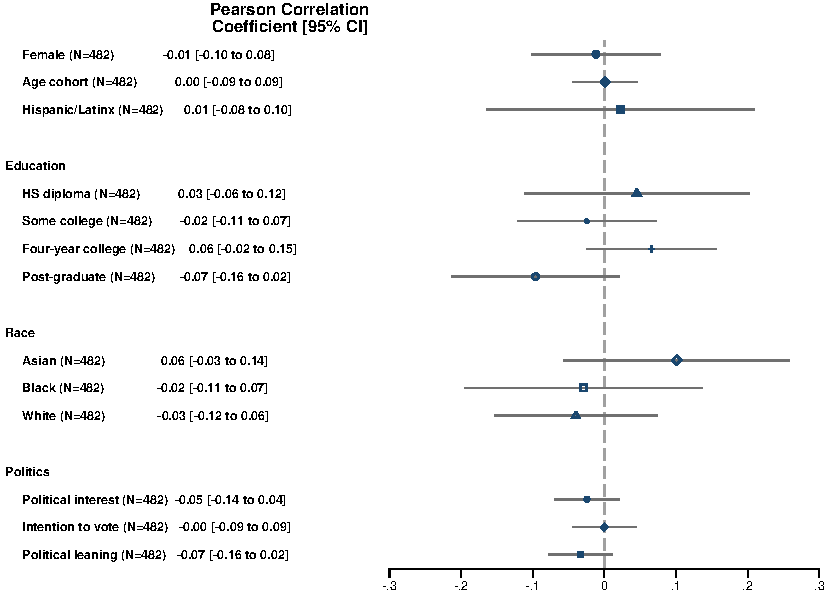
\includegraphics[scale=.8]{../figs/baltest-24k-rw.pdf}
  \label{fig:baltest-24k-rw}
  \caption*{\footnotesize Figure shows the results from a balance test for the Amazon Mechanical Turk sample. Self-reported characteristics of respondents are compared between the respondents assigned to the 24k arm and the RW arm as described in \nameref{sec:data}.
  Rows are self-reported characteristics.
  Second column reports the correlation between characteristics and the 24k arm, and the 95\% confidence intervals constructed from bootstrapped standard errors (n=10,000).
  Third column reports the estimated difference between the 24k respondents and the RW respondents.
  Horizontal bars are 95\% confidence intervals constructed from robust standard errors.
  }
\end{figure}
\end{center}


\begin{figure}[ht]
	\caption{Partisan Knowledge Gaps with Partisan Cues: YouGov}
	\centering
	\begin{subfigure}{.495\textwidth}\centering
		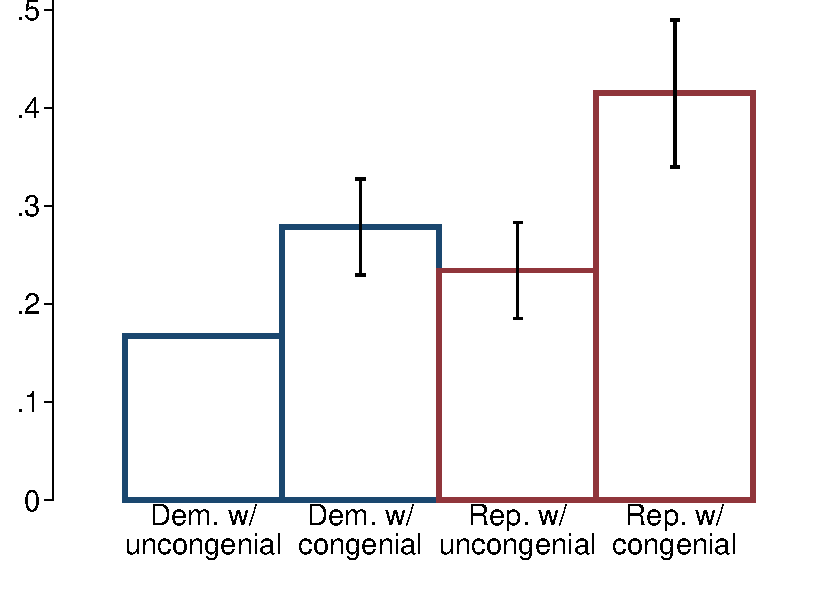
\includegraphics[width=\textwidth]{../figs/yougov-unemp-congenialcue-partisan.pdf}
		\caption{Unemployment}
	\end{subfigure}
	\hfil
	\begin{subfigure}{.495\textwidth}\centering
		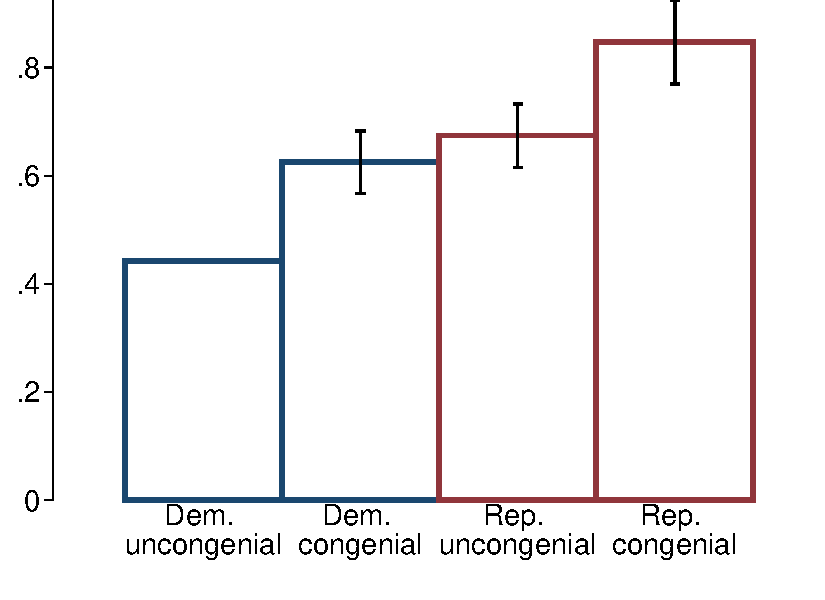
\includegraphics[width=\textwidth]{../figs/yougov-deficit-congenialcue-partisan.pdf}
		\caption{Budget deficit}
	\end{subfigure}
	\caption*{\footnotesize Figure shows the effect of congenial cues for the YouGov survey by partisanship. Bars indicate the predicted percent of responses saying that unemployment have gone up (correct response) as retrieved from the estimates in \cref{tab:partisangaps-yougov} (columns (2) and (5)).  The estimates are obtained by estimating:\\

	$\qquad\text{correct response}_{i} = \alpha + \beta (congenial \; cue)_i + \gamma (Rep)_i + \delta (congenial\; cue \times Rep)_i + \varepsilon_{i}$.\\

	Capped vertical bars indicate 95\% confidence intervals.
	}
	\label{fig:yougov-reg-by-partisanship}
\end{figure}

\clearpage
\section{Item Text for the MTurk Study}\label{si:mturk}

\textbf{Preface for Different Conditions}

\textbf{RW, IP}\newline
Now here are some questions about what you may know about politics and public affairs.

\textbf{FSR, 14k, 24k}\newline
Now here are some questions about what you may know about politics and public affairs.
We are interested in measuring what people currently know and can recall on their own and are
just as interested in what people don't know as in what they do know. So we'd like your
agreement to just say ``don't know'' if you don't know the answer—without looking anything up
or talking with anyone about it.

\textbf{Item Text}
\textbf{24k}\newline
Now here are a series of statements. On a scale of 0 to 10, where 0 means definitely false,
10 means definitely true, and 5 is exactly in the middle, how definitely true or false is
each statement?

\begin{itemize}
	\item Barack Obama was born in the US (T)
	\item  Barack Obama is a Muslim (F)
	\item  The Affordable Care Act gives illegal immigrants financial help to buy health insurance (F)
	\item  The Affordable Care Act does not create government panels to make decisions about end-of-life care (T)
	\item  Temperatures around the world are increasing because of human activity, like burning coal and gasoline (T)
	\item  Most climate scientists believe that global warming is not occurring (F)
	\item  In the 2016 presidential election, President Trump won the majority of the legally cast votes (F)
	\item  The vaccine for measles, mumps, and rubella (MMR) causes autism in children. (F)
	\item  Since 2012, the annual federal budget deficit has increased. (T)
\end{itemize}

\textbf{Rest of the Conditions, By Item}

\begin{itemize}
\item Obama's Birthplace

\textbf{RW and IP}\newline

According to the Constitution, American presidents must be ``natural born citizens.''
Some people believe Barack Obama was not born in the United States, but was born
in another country. Do you think Barack Obama was born in ...?
\begin{itemize}
	\item The US
	\item Another country
\end{itemize}

\textbf{FSR}\newline
Some people believe Barack Obama was not born in the United States, but was born
in another country. Was he born in ...?
\begin{itemize}
	\item The US
	\item Another country
	\item DK (plus DK pref)
\end{itemize}

\textbf{14k}\newline

Was Barack Obama born in ...?
\begin{itemize}
	\item the US
	\item Another country
	\item DK (plus DK pref)
\end{itemize}

\item Obama Religion\newline
\textbf{RW}\newline

Do you personally believe that Barack Obama is a ...?
\begin{itemize}
	\item Muslim
	\item Christian
\end{itemize}

\textbf{IP}\newline

Most people have a religion. Some people believe Barack Obama is a Muslim. Do
you personally believe that Barack Obama is a \ldots?
\begin{itemize}
	\item Muslim
	\item Christian
\end{itemize}

\textbf{FSR}\newline

Some people believe Barack Obama is a Muslim. Is he a \ldots?
\begin{itemize}
	\item Muslim
	\item Christian
	\item DK (+ DK pref)
\end{itemize}

\textbf{14k}\newline

Is Barack Obama a \ldots?
\begin{itemize}
	\item Muslim
	\item Christian
	\item DK (plus DK pref)
\end{itemize}

\item ACA Illegal\newline
\textbf{RW}\newline

To the best of your knowledge, would you say the Affordable Care Act\ldots?
\begin{itemize}
	\item Gives illegal immigrants financial help to buy health insurance
	\item Does not give illegal immigrants financial help to buy health insurance
\end{itemize}

\textbf{IP}\newline

As you may know, there is currently talk of changing the Affordable Care Act
(ACA), enacted in 2010. Some people believe that the ACA gives illegal immigrants
financial help to buy health insurance. To the best of your knowledge, would you say
the ACA\ldots?
\begin{itemize}
	\item Gives illegal immigrants financial help to buy health insurance
	\item Does not give illegal immigrants financial help to buy health insurance
\end{itemize}

\textbf{FSR}\newline

Some people believe that Affordable Care Act gives illegal immigrants financial help
to buy health insurance. Does the Affordable Care Act\ldots?
\begin{itemize}
	\item Give illegal immigrants financial help to buy health insurance
	\item Not give illegal immigrants financial help to buy health insurance
	\item DK (+ DK pref)
\end{itemize}

\textbf{14k}\newline
Does the Affordable Care Act\ldots?
\begin{itemize}
	\item Give illegal immigrants financial help to buy health insurance
	\item Not Give illegal immigrants financial help to buy health insurance
	\item Don't know (+ DK pref)
\end{itemize}

\item ACA—Death Panels\newline
\textbf{RW}\newline
To the best of your knowledge, would you say that the Affordable Care Act \ldots?
\begin{itemize}
	\item Creates government panels to make decisions about end-of-life care
	\item Does not create government panels to make decisions about end-of-life care
\end{itemize}

\textbf{IP}\newline

Some people believe that Affordable Care Act establishes a government panel to
make decisions about end-of-life care. To the best of your knowledge, would you say
that the Affordable Care Act \ldots?
\begin{itemize}
	\item Creates government panels to make decisions about end-of-life care
	\item Does not create government panels to make decisions about end-of-life care
\end{itemize}

\textbf{FSR}\newline

Some people believe that Affordable Care Act establishes a government panel to
make decisions about end-of-life care. Does the Affordable Care Act\ldots?
\begin{itemize}
	\item Creates government panels to make decisions about end-of-life care
	\item Does not create government panels to make decisions about end-of-life care
	\item DK (+ DK pref)
\end{itemize}

\textbf{14k}\newline
Does the Affordable Care Act \ldots?
\begin{itemize}
	\item Creates government panels to make decisions about end-of-life care
	\item Does not create government panels to make decisions about end-of-life care
	\item DK (+ DK pref)
\end{itemize}

\item Global Warming—Happening + Causes\newline
\textbf{RW}\newline
Which of the following best fits your view about this? Are temperatures around the
world \ldots?
\begin{itemize}
	\item Increasing because of natural variation over time, such as produced the ice age
	\item Increasing because of human activity, like burning coal and gasoline
	\item Staying about the same as they have been
\end{itemize}

\textbf{IP}\newline
Recently, you may have noticed that global warming has been getting some attention
in the news. Some people believe that temperatures are increasing around the world
because of natural variation over time, such as produced the ice age. Which of the
following best fits your view about this? Would you say that temperatures around the
world are\ldots?
\begin{itemize}
	\item Increasing because of natural variation over time, such as produced the ice age
	\item Increasing because of human activity, like burning coal and gasoline
	\item Staying about the same as they have been
\end{itemize}

\textbf{FSR}\newline

Some people believe that temperatures are increasing around the world because of
natural variation over time, such as produced the ice age. Are temperatures around
the world \ldots?
\begin{itemize}
	\item Increasing because of natural variation over time, such as produced the ice age
	\item Increasing because of human activity, like burning coal and gasoline
	\item Staying about the same as they have been
	\item DK (+ DK pref)
\end{itemize}

\textbf{14k}\newline
Are temperatures around the world \ldots?
\begin{itemize}
	\item Increasing because natural variation over time, such as produced the ice age
	\item Increasing because human activity, like burning coal and gasoline
	\item Staying about the same as they have been
	\item DK (+ DK pref)
\end{itemize}

\item GW—Scientist Agreement\newline
\textbf{RW}\newline
Just your impression, which one of the following statements do you think is most
accurate?
\begin{itemize}
	\item Most climate scientists believe that global warming is occurring.
	\item Most climate scientists believe that global warming is not occurring.
	\item Climate scientists are about equally divided about whether global warming is occurring or not
\end{itemize}

\textbf{IP}\newline
As you may know, the term ``global warming'' refers to the claim that temperatures
have been increasing around the world. Some people believe that most climate
scientists believe that global warming is not occurring. Just your impression, which
one of the following statements do you think is most accurate?
\begin{itemize}
	\item Most climate scientists believe that global warming is occurring.
	\item Most climate scientists believe that global warming is not occurring.
	\item Climate scientists are about equally divided about whether global warming is occurring or not
\end{itemize}
\textbf{FSR}\newline
Some people believe that most climate scientists believe that global warming is not
occurring. Which one of the following statements is most accurate?
\begin{itemize}
	\item Most climate scientists believe that global warming is occurring.
	\item Most climate scientists believe that global warming is not occurring.
	\item Climate scientists are about equally divided about whether global warming is occurring or not
	\item DK (+ DK pref)
\end{itemize}

\textbf{14k}\newline
Which one of the following statements is most accurate?
\begin{itemize}
	\item Most climate scientists believe that global warming is occurring.
	\item Most climate scientists believe that global warming is NOT occurring.
	\item Climate scientists are about equally divided about whether global warming is occurring or not
	\item DK (+ DK pref)
\end{itemize}

\item Voter Fraud\newline
\textbf{RW}\newline
As you may know, President Trump has said that several million people voted
illegally in the 2016 presidential election and that he won the majority of the legally
cast votes. Do you believe that President Trump \ldots?
\begin{itemize}
	\item Won the majority of the legally cast votes
	\item Did not win the majority of the legally cast votes
\end{itemize}

\textbf{IP}\newline
As you may know, not everyone living in the US has the legal right to vote. President
Trump has said that several million people voted illegally in the 2016 presidential
election and that he won the majority of the legally cast votes. Do think that that
President Trump \ldots?
\begin{itemize}
	\item Won the majority of the legally cast votes
	\item Did not win the majority of the legally cast votes
\end{itemize}

\textbf{FSR}\newline
As you may know, President Trump has said that several million people voted
illegally in the 2016 presidential election and that he won the majority of the legally
cast votes. Did President Trump \ldots?
\begin{itemize}
	\item Won the majority of the legally cast votes
	\item Did not win the majority of the legally cast votes
	\item DK (+ DK pref)
\end{itemize}

\textbf{14k}\newline
In the 2016 presidential election, did President Trump \ldots?
\begin{itemize}
	\item Won the majority of the legally cast votes
	\item Did not win the majority of the legally cast votes
	\item DK (+ DK pref)
\end{itemize}

\item Vaccines\newline
\textbf{RW}\newline
From what you have read or heard, do you personally think that the vaccine for
Measles, Mumps, and Rubella (MMR):
\begin{itemize}
	\item Causes autism in children
	\item Does not cause autism is children
\end{itemize}

\textbf{IP}\newline
As you may know, most children receive the vaccine for Measles, Mumps, and
Rubella (MMR). Some people believe that the MMR vaccine causes autism in
children. From what you have read or heard, do you personally think that the MMR
vaccine:
\begin{itemize}
	\item Causes autism in children
	\item Does not cause autism is children
\end{itemize}

\textbf{FSR}\newline
Some people believe that the vaccine for Measles, Mumps, and Rubella (MMR)
causes autism in children. Does the MMR vaccine \ldots?
\begin{itemize}
	\item Cause autism in children
	\item Not cause autism in children.
	\item DK (+ DK pref)
\end{itemize}

\textbf{14k}\newline
Does the vaccine for Measles, Mumps, and Rubella (MMR) \ldots?
\begin{itemize}
	\item Cause autism in children
	\item Not cause autism in children.
	\item DK (+ DK pref)
\end{itemize}

\item Obama—Budget Deficit\newline
\textbf{RW}\newline
As you may know, the federal government runs a deficit when it spends more than it
takes in. Since 2012, would you say that the annual federal budget deficit has \ldots
\begin{itemize}
	\item Increased
	\item Stayed about the same
	\item Decreased
\end{itemize}

\textbf{IP}\newline
As you may know, the federal government runs a deficit when it spends more than it
takes in. Since 2012, with the Republicans having the majority in the U.S. House of
Representatives, would you say that the annual federal budget deficit has \ldots
\begin{itemize}
	\item Increased
	\item Stayed about the same
	\item Decreased
\end{itemize}

\textbf{FSR}\newline
Since 2012, with the Republicans having the majority in the U.S. House of
Representatives,
\begin{itemize}
	\item has the annual federal budget deficit \ldots.
	\item Increased
	\item Stayed about the same
	\item Decreased
	\item DK (+ DK pref)
\end{itemize}

\textbf{14k}\newline

Since 2012, has the annual federal budget deficit \ldots
\begin{itemize}
	\item Increased
	\item Stayed about the same
	\item Decreased
	\item DK (+ DK pref)
\end{itemize}
\end{itemize}

\newpage




\clearpage
\section{Item Text for the Second MTurk Study}\label{si:mturk2}


The second Amazon MTurk survey was fielded in April 2017 and had 1,059 participants. In this survey we made use of new questions and probes to examine the effect of question design on (partisan) knowledge. We asked the participants four questions about the Affordable Care Act (2), the effect of greenhouse gases (1), and Donald Trump's recent executive order on immigration (1).

\begin{comment}
\noindent
\textbf{Rules for Coding Open Ended Questions}\newline

In coding open-ended responses, all misspellings, modifications, synonyms, and identifiable abbreviations of a word were fully credited.


\noindent
\textbf{Honesty Pledge}

At the beginning of the survey, a random two-thirds of the respondents were asked to commit to not look up the answers or to ask anyone about the answers. Rest one-third of the participants didn’t see any message at the start.


\noindent
\textbf{Photo Vs. Text}

Individuals were asked knowledge questions about domestic and international political leaders. These leaders were presented to the participants either as a photo (asking for name or position) or they saw the name as text (asking for the position).

\noindent
The preamble for the two treatments were:

\begin{description}
\item[Photo:] Here’s a set of photos. For each photo, can you tell me what position he or she holds? If you don’t know, don’t worry about it. Just leave the space blank, and move on to the next person. What position does this person hold?
  \item[Text:] Here’s a list of names. For each name, can you tell me what position that person holds? If you don’t know, don’t worry about it. Just leave the space blank, and move on to the next person. What position does this person hold?
\end{description}


\begin{itemize}
\item Mitch McConnell
  \begin{itemize}
\item  OE: (Senate OR majority) AND (leader OR chief OR head OR president OR chair OR whip)
\end{itemize}
\item Chuck Schumer
  \begin{itemize}
\item  OE: (Senate OR minority) AND (leader OR in charge)
\end{itemize}
\item Angela Merkel
    \begin{itemize}
\item OE: German AND (President OR Leader OR Prime Minister OR Chancellor OR Premier AND Ruler AND charge)
\end{itemize}
\item Vladimir Putin
  \begin{itemize}
\item OE: Russia AND (President OR Leader OR Head OR Chancellor OR Premier OR Prime Minister)
\end{itemize}
\item John Roberts
  \begin{itemize}
\item OE: Chief AND Justice
\end{itemize}
\item Nancy Pelosi
  \begin{itemize}
\item OE: Minority AND Leade
\end{itemize}
\end{itemize}

\end{comment}

One half of the survey respondents got a conventional closed-ended item with five options including the opportunity to mark Don’t know. The other half of the respondents had to assess the truth of statements on a scale from definitely false (0) to definitely true (10).


\begin{description}
\item[1.] Does the Affordable Care Act ...?
  \begin{itemize}
    \item  CE: Provide coverage for people who are currently in the country illegally, Replace private health insurance with a ``single payer system'', \textbf{Increase the Medicare payroll tax for upper-income Americans}, Reimburse routine mammograms only for women older than 50, Don’t know (5)
    \item  Scale: Rating each response option above from definitely false (0) to definitely true (10). Don’t know was not included. See Figure \ref{fig:aca1}.
    \end{itemize}
    \item[2.] Are greenhouse gases ...?
  \begin{itemize}
  \item CE: A cause of respiratory problems, A cause of for lung cancer, Damaging the ozone layer, \textbf{A cause of rising sea levels}, or Don’t know
  \item Scale: Rating each response option above from definitely false (0) to definitely true (10). Don’t know was not included. See Figure \ref{fig:gg1}.
    \end{itemize}
  \item[3.] And does the Affordable Care Act ...?
    \begin{itemize}
  \item CE: Create government panels to make end-of-life decisions for people on Medicare, Replace Medicare with a ``public option'', \textbf{Limit future increases in payments to Medicare providers}, Cut benefits to existing Medicare patients, Don’t know
  \item Scale: Rating each response option above from definitely false (0) to definitely true (10). Don’t know was not included. See Figure \ref{fig:aca2}.
    \end{itemize}
        \item[4.] Does President Trump’s most recent executive order on immigration ...?
  \begin{itemize}
  \item  CE: Subject immigrants living in the U.S. illegally to deportation, Strip immigrants from countries supporting terrorism of their green cards, Strip immigrants from several Muslim-majority countries of their green cards, \textbf{Temporarily ban immigrants from several majority-Muslim countries}, Don’t know
    \item  Scale: Rating each response option above from definitely false (0) to definitely true (10). Don’t know was not included. See Figure \ref{fig:eo1}.
    \end{itemize}
    \end{description}

If the close-ended questions 3 and 4 were not answered with Don’t know the respondents received one of two a follow- up question:
\begin{itemize}
\item OE: What made you choose that response?
 \item CE: What made you choose that response? I asked someone I know, I looked it up, I’ve read, seen, or heard that, It makes me feel good to think that, It makes sense, in view of other things I know, I just thought I’d take a shot
\end{itemize}

\begin{center}
	\begin{figure}[H]
		\centering
		\caption{Affordable Care Act 1 Scale Question}
		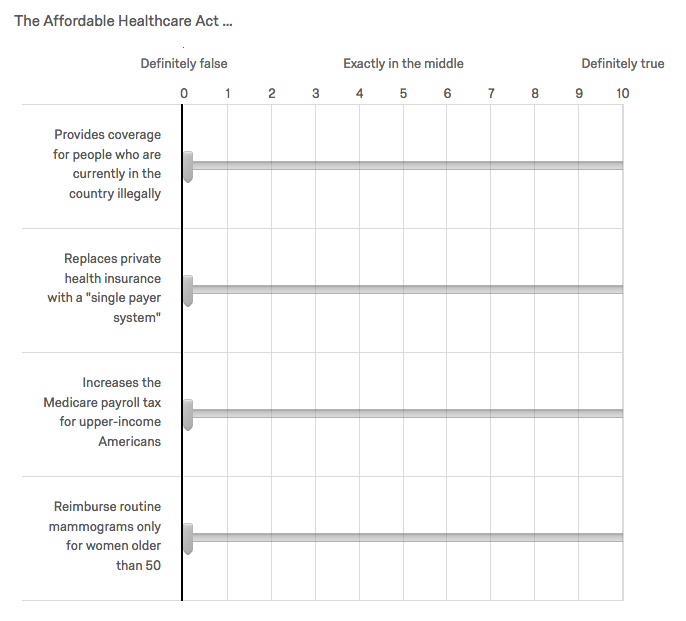
\includegraphics[width=\textwidth]{../figs/hk_aca1.png}
		\label{fig:aca1}
		\caption*{\footnotesize }
	\end{figure}
\end{center}


\begin{center}
	\begin{figure}[H]
		\centering
		\caption{Greenhouse Gases Scale Question}
		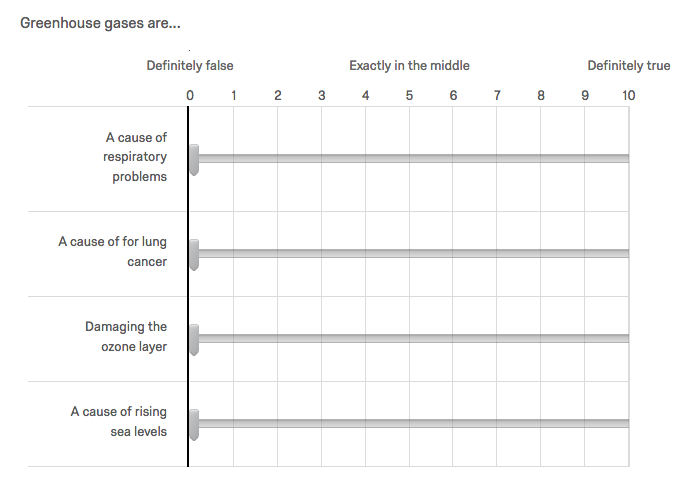
\includegraphics[width=\textwidth]{../figs/hk_gg1.png}
		\label{fig:gg1}
		\caption*{\footnotesize }
	\end{figure}
\end{center}


\begin{center}
	\begin{figure}[H]
		\centering
		\caption{Affordable Care Act 2 Scale Question}
		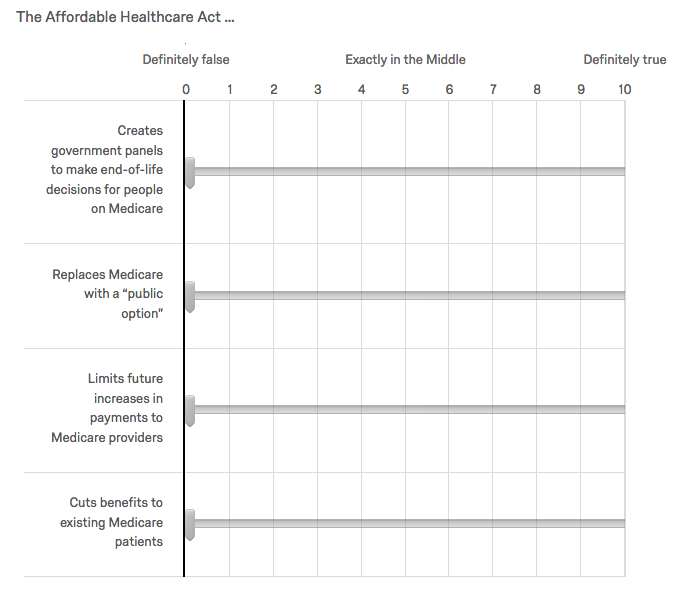
\includegraphics[width=\textwidth]{../figs/hk_aca2.png}
		\label{fig:aca2}
		\caption*{\footnotesize }
	\end{figure}
\end{center}


\begin{center}
	\begin{figure}[H]
		\centering
		\caption{Executive Order Scale Question}
		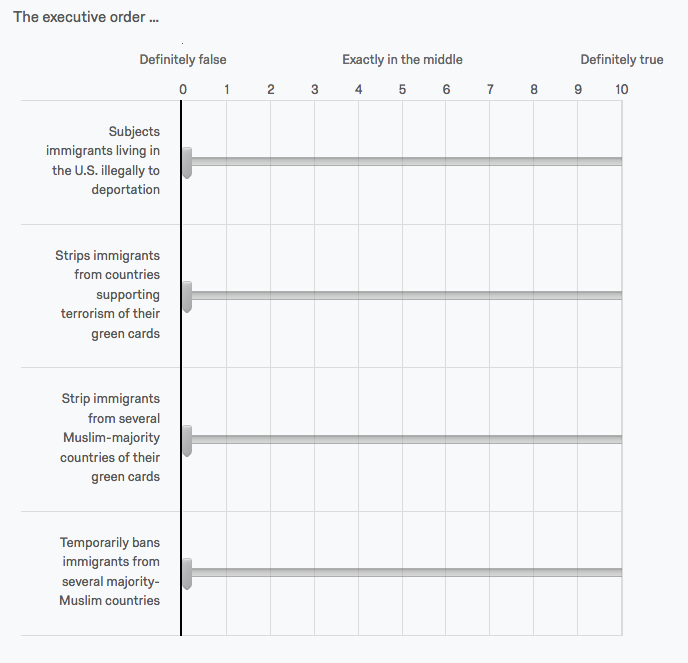
\includegraphics[width=\textwidth]{../figs/hk_eo1.png}
		\label{fig:eo1}
		\caption*{\footnotesize }
	\end{figure}
\end{center}

\newpage

\noindent
\textbf{Inference}

The following close-ended two deficit related questions were presented to all survey participants.

\begin{enumerate}
    \item During the time Barack Obama was president, the federal deficit: \textbf{Increased}, Remained about the same, Decreased, Don’t Know
    \item During the time George W. Bush was president, the federal deficit: \textbf{Increased}, Remained about the same, Decreased, Don’t Know
\end{enumerate}

Both questions were followed by a probe. For one half of the respondents this probe was open and for the other one the probe was closed.
\begin{itemize}
 \item OE: What made you choose that response?
 \item CE: What made you choose that response? I asked someone I know, I looked it up, I’ve read, seen, or heard that, It makes me feel good to think that, It makes sense, in view of other things I know, I just thought I’d take a shot
\end{itemize}
